\chapter{\label{sec:litreview}The State of the Art}

In order to develop new methods to ease the model creation process, we must first understand the efforts that have already taken place in the field. We must understand the scanning and modelling process, and how models will be animated once they have been created. In this chapter, we will review current methods of model creation and animation, as well as related areas such as surface representation and compression. This is an area with a large commercial element, so we must understand not only academic research into these fields, but also commercially-available hardware and software systems. 

We start by examining systems for capturing detailed surface measurements from physical objects, and then review the possible representations in which this data can be stored. We are particularly interested in highly detailed surfaces, and therefore review a number of methods for representing such surfaces in an efficient manner, including methods of compressing this data. We also wish to animate the models that we will create, and so we end by reviewing current methods of mesh animation.

This review does not aim to be exhaustive, due to the wide range of material covered, but instead aims to highlight major approaches in order to provide an overview of the field.

\section{\label{sec:litreview:scanning}3D Scanning Systems}
In  this research, we wish to represent detailed models in an efficient manner. We must therefore discuss how such models are obtained. This can be done either by creating an object on a computer from scratch, using tools like 3D Studio MAX \cite{3DSMAX} or Maya \cite{Maya}, or it can begin with a physical object in the real world. In this case, a digitised model of the physical object must be created.

The first stage in any 3D scanning system is the capture of surface data from the physical object, the scanning or sensing phase \cite{Isdale98}. This involves using some form of hardware system to measure the surface of the object. Such systems fall into three main categories; tracking, imaging and range finding.

\subsection{\label{sec:litreview:scanning:tracking}Tracking}
Tracking systems typically capture data by positioning a probe on the surface of the object and capturing a single 3D point at a time. For instance, Coordinate Measuring Machines (CMMs) consist of a probe attached to a mechanical arm, which contains sensors that precisely measure the position of the probe when a point is captured. Other systems use different methods of tracking to provide greater freedom, such as electromagnetic and ultrasonic trackers. Such manual capture systems can be extremely time-consuming, as each point in the final model needs to be captured individually.

\subsection{\label{sec:litreview:scanning:imaging}Imaging}
Imaging systems take a number of 2D images of an object, normally from different angles, which are then processed to calculate 3D surface data. Imaging systems range from systems that generate point clouds by calculating range measurements, to systems that generate models directly by extracting feature points from the image data. Other systems use the silhouette of the object to create a volumetric model which can then be converted into a polygonal representation. Medical scanners also come under the heading of imaging systems, using sensors such as MRI, CT and so on \cite{Short02}.

\subsection{\label{sec:litreview:scanning:range}Range Finding}
Range finding systems generally produce a 2D array of distance measurements known as a {\it range image}, which can be easily converted into a mesh. The most common type of range finding systems are laser scanners, which project a laser stripe onto the surface being scanned, and capture the shape of the stripe through a camera positioned at an angle to the laser. This can be converted into a set of distance measurements, in a process known as {\it optical triangulation}. Some systems are also capable of capturing texture information from objects, which can then be mapped onto the generated models. 

A popular technique is to combine a tracking system and a range finder. Systems of this kind include 3D Scanner's ModelMaker \cite{3DScanners}, which uses a CMM arm with an attached laser scanner, and the Polhemus HLS \cite{Polhemus}, which uses Polhemus' magnetic tracking system with a laser scanner. This type of system allows the scanner to be moved freely around an object, while capturing position and orientation information for the scanner itself. Some scanners, such as those from \citet{Cyberware}, move a laser scanner around the object automatically, but this requires a large working area and complex machinery. 

Such systems generally produce very dense, unstructured surface data, which is very difficult to work with. In order to be usable, this data must be processed into a more easily manipulated format.

\section{\label{sec:litreview:surfaces}Surface Representations}
\begin{figure}
\begin{center}
\begin{tabular}{ccc}
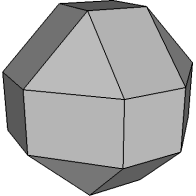
\includegraphics[width=3.5cm]{../images/polymesh} &
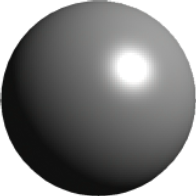
\includegraphics[width=3.5cm]{../images/quadric} &
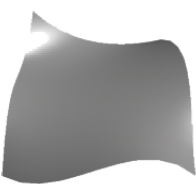
\includegraphics[width=3.5cm]{../images/nurbs} \\
{\it(a)} & {\it(b)} & {\it(c)}
\end{tabular}
\caption[Surface Representations]{\label{fig:surfaces} Surface Representations. (a) Polygonal Mesh. (b) Quadric Ellipsoid. (c) NURBS Surface.}
\end{center}
\end{figure}
In order to represent an object in a computer, we must store data about its surface in some form or another. There are a number of possible surface representations we can choose from, each with their own advantages and disadvantages.

\subsection{\label{sec:litreview:surfaces:polygon}Polygonal Surfaces}

Polygonal models represent a surface using a set of planar polygons, usually triangles or quadrilaterals, as shown in figure \ref{fig:surfaces}a. These surfaces are the the dominant form of representation in 3D graphics, particularly at the consumer level, where much effort has been expended to create hardware that can render polygonal models as fast as possible. However, with the desire for increasingly realistic graphics, their limitations have become clear.

Polygonal models can approximate surfaces of arbitrary complexity, but as they are piecewise linear, they cannot truly represent curved surfaces \cite{Besl94}. Even a close approximation to the surface would require a large number of polygons.

\subsection{\label{sec:litreview:surfaces:smooth}Smooth Surfaces}

Many surfaces that we wish to model are curved and, as noted above, accurately representing a curved surface with a polygonal model would require a large number of polygons. Instead, we can use {\it smooth} surfaces to represent such models. Unlike polygonal models, smooth surfaces are not piecewise linear, so are capable of representing curved surfaces efficiently.

\subsubsection{\label{sec:litreview:surfaces:smooth:polynomial}Polynomial Surfaces}

Most 3D rendering packages include support for {\it polynomial} surfaces, which result from the evaluation of a polynomial function in terms of spatial coordinates. The order of the polynomial defines the smoothness of the surface. First-order polynomials define planar C0 surfaces, and second-order polynomials define C1 {\it quadric} surfaces such as ellipsoids and paraboloids (see figure \ref{fig:surfaces}b). Cubic and quartic surfaces are also common. This form of representation is limited to representing the surfaces that can be represented by a polynomial equations, however, and cannot represent surfaces of arbitrary geometry and topology.

\subsubsection{\label{sec:litreview:surfaces:smooth:curved}Curved Surface Patches}

Curved surface patches are a generalisation of smooth 2D curves to three dimensions. The surface is generally a quadrilateral patch whose geometry is defined by a number of control points. Due to the fact that curved surfaces can only represent quadrilateral patches, modelling of complex objects requires the use of multiple patches, which must be held together, or {\it stitched}, so that cracks do not appear during animation.

Two dimensional smooth curves use a polynomial function to define the shape of the curve. The coefficients of the polynomial are the {\it control points} of the curve. Two of the more popular types of curve are {\it Bezier} and {\it B-Spline} curves, both defined by a cubic polynomial. In a Bezier curve, two control points define endpoints, while another two control the shape of the curve between the points. The cubic B-Spline is a generalisation of the Bezier curve, and defines the curve its two innermost control points, using the other two to control endpoint gradients. Using B-Splines, a curve with an arbitrary number of control points can be specified by stitching B-Spline curve segments together. If the control points for one B-Spline overlap the control points for the next, the two will be C2 continuous at the join.

\citet{Forsey88} describe an extension to B-Spline surfaces, the {\it Hierarchical B-Spline patch}. These patches can be refined as required (for instance in areas of high surface detail) by adding extra control points, creating a higher-order surface in the local area.

\subsubsection{\label{sec:litreview:surfaces:smooth:nurbs}NURBS Patches}

Non-Uniform Rational B-Splines (NURBS), illustrated in figure \ref{fig:surfaces}c, are a general form of B-Spline, and are now a popular representation for curves and surfaces. They have two properties over normal B-Splines that make them particularly popular. Firstly, both NURBS and B-Splines can be subjected to affine transformations without distortion. However, perspective transformations are not affine, and B-Splines do not appear correctly under perspective viewing. NURBS, however, do not suffer from this, and appear as intended even after non-affine transformation, a vital property for 3D graphics. Secondly, quadric surfaces can only be approximated by standard B-Splines, but can be shown to be a special case of NURBS.

\subsubsection{\label{sec:litreview:surfaces:smooth:implicit}Implicit Surfaces}

An implicit surface is not defined by explicit evaluation of an equation, or by a set of 3D points, but as the set of solutions to a function of the form $f(x,y,z) = a$. The surface itself is a contour or {\it isosurface} in the 3D scalar field defined by the function, and upon which the result of the equation is some constant value $a$ (normally 0). For rendering purposes, implicit surfaces can be {\it tiled}, or converted into a polygonal representation \cite{Ning93}.

\subsubsection{\label{sec:litreview:surfaces:smooth:subdivision}Subdivision Surfaces}
Recently, {\it subdivision} surfaces have gained popularity, and have been incorporated into a number of rendering packages. Subdivision surfaces bridge the gap between polygonal and smooth surfaces, by using an arbitrary polygonal mesh to define a parametric surface. The subdivision surface is created by repeated application of a subdivision algorithm to the polygonal control mesh. The limit of this process defines a smooth spline surface. There are a number of different types of subdivision surface, each with its own subdivision algorithm and restrictions on control mesh structure. The major types are Doo-Sabin \cite{Doo78}, Catmull-Clark \cite{Catmull78}, Loop \cite{Loop94} and Butterfly \cite{Dyn90} surfaces. 

\begin{figure}
\begin{center}
\begin{tabular}{cccc}
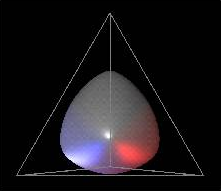
\includegraphics[width=3.18cm]{../images/tetra_doosabin} &
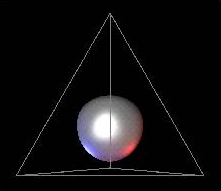
\includegraphics[width=3.18cm]{../images/tetra_catmullclark} &
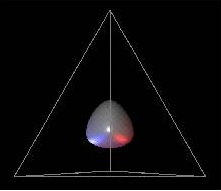
\includegraphics[width=3.18cm]{../images/tetra_loop} &
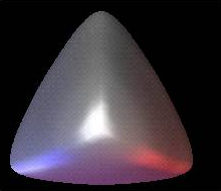
\includegraphics[width=3.18cm]{../images/tetra_butterfly} \\
{\it(a)} & {\it(b)} & {\it(c)}  & {\it(d)}
\end{tabular}
\caption[Subdivision Surfaces]{\label{fig:subdivision} Subdivision Surfaces. (a) Doo-Sabin subdivision. (b) Catmull-Clark subdivision. (c) Loop subdivision. (c) Butterfly subdivision. Images taken from \cite{Zorin99}.}
\end{center}
\end{figure}

Doo-Sabin subdivision, shown in figure \ref{fig:subdivision}a, is a {\it dual} subdivision method based on quadratic uniform B-Spline surfaces. Each level of subdivision divides each vertex into {\it n} new vertices, where {\it n} is the number of faces adjacent to the vertex. The new positions of the new vertices are calculated as the average of the original vertex, the centroid of the face, and the midpoints of the two edges adjacent to the face and the original vertex.

Catmull-Clark surfaces (shown in figure \ref{fig:subdivision}b) are based on the subdivision of cubic uniform B-Spline surfaces, and create a three kinds of new vertices at each subdivision step. New points are added in the centre of the faces of the control mesh, and at the midpoints of control mesh edges. The control mesh vertices are also affected by the subdivision.

Both of the above subdivision schemes use control meshes of arbitrary topology. Loop subdivision (see figure \ref{fig:subdivision}c) however, uses control meshes composed only of triangles. At each level, each triangular face is divided into four smaller faces, and smoothed based on the subdivision of quartic uniform box splines.

All of the above schemes use an {\it approximating} subdivision scheme, in which the original control vertices do not necessarily lie on the limit surface. Butterfly subdivision, illustrated in figure \ref{fig:subdivision}d, is an {\it interpolating} scheme, in which original control points are preserved on the limit surface. Like Loop, Butterfly subdivision works on a control mesh composed of triangular faces.

Subdivision surfaces can be extended to allow sharp edges by constraining the subdivision routine. \citet{Hoppe94a} proposed such a method for Loop surfaces, and \citet{DeRose98} have developed a similar method for Catmull-Clark surfaces.

\subsection{\label{sec:litreview:surfaces:detail}Representation of Surface Detail}
\begin{figure}
\begin{center}
\begin{tabular}{ccc}
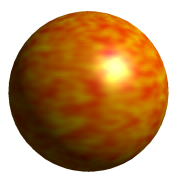
\includegraphics[width=3.5cm]{../images/sphere_texmap} &
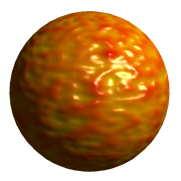
\includegraphics[width=3.5cm]{../images/sphere_bumpmap} &
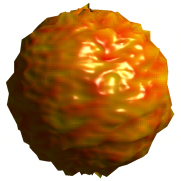
\includegraphics[width=3.5cm]{../images/sphere_dispmap} \\
{\it (a)} & {\it (b)} & {\it (c)} \\
\end{tabular}
\caption[Surface Detail]{\label{fig:surfacedetail} Surface Detail. (a) Texture mapping. (b) Bump mapping. (c) Displacement mapping.}
\end{center}
\end{figure}
A polygonal or smooth surface can represent the general shape of an object efficiently, but realistic objects possess fine surface details, such as wrinkles in skin. Unless the model is extremely detailed, these are impossible to represent, as well as difficult to edit. A polygonal model would require a very large number of faces to represent small surface details, and a smooth surface would need either a large number of patches or a very high order polynomial. Both of these will increase rendering time, and therefore prohibit interactive animation. A number of techniques have therefore been developed to create the illusion of a detailed surface without requiring complex geometry.

The simplest of these is {\it texture mapping}, shown in figure \ref{fig:surfacedetail}a, where a 2D image of the surface of the real object is mapped onto the surface of the model. This gives the appearance of surface detail, but has a limitation in that the texture will not change under different lighting conditions. The underlying geometry of the surface is also visible when examined closely.

A more realistic appearance can be created by {\it bump mapping}, proposed by \citet{Blinn78}, which applies details during shading of the surface. A bump map is a texture used to perturb the normal of the surface during shading. This changes the lighting on the surface, making it appear as if the surface detail is actually present. The surface itself is still the original shape, as can be seen from the object's silhouette.

The most realistic results are obtained using {\it displacement mapping}, originally proposed by \citet{Cook84}. Displacement mapping is a step beyond bump and texture mapping in that it actually perturbs the geometry of the surface it is applied to. A displacement map is generally an image where each pixel encodes an offset along the surface normal, which is mapped onto the surface. During rendering, a new surface is created which includes all of the surface detail from the displacement map. As this approach actually changes the surface geometry, the result is indistinguishable from a very detailed mesh. However, displacement maps are currently very expensive to compute, and while they have been used in film production for a reasonable length of time, until recently they have been of limited use for real-time applications. However, the power of consumer graphics cards is now such that current graphics APIs include displacement map support \cite{DirectX9}, and hardware support will not be far behind. The use of displacement maps for modelling is discussed further in section \ref{sec:litreview:modeling:detail}.

\section{\label{sec:litreview:reconstruction}Surface Reconstruction}

After surface measurements of an object have been taken, we must convert these measurements into a form that we can use, such as those mentioned above in section \ref{sec:litreview:surfaces}.

In many cases, the surface data will be in the form of a set of range images that must be fused into a single surface. There are two main problems involved in merging multiple range images \cite{Illingworth98}. The first is the problem of {\it registration}, which involves positioning the range images correctly relative to each other. When multiple range images are taken without information on the sensor position for each one, this is a major problem \cite{Besl92}. However, the combination tracker/scanner systems avoid this problem, as the scanner position is always known. In these cases, we only have to solve the second problem, how to fuse the multiple range images together into a single surface.

Early approaches to this problem concentrated on fitting deformed polynomial surfaces such as planes and spheroids to the range data. These methods have their obvious limitations, being confined to the reconstruction of surfaces with the same topology as the polynomial surface.

\subsection{\label{sec:litreview:reconstruction:fusion}Mesh Fusion}

An early attempt at a solution using triangulated meshes was proposed by \citet{Turk94}, who developed a method that triangulated individual range images into a set of polygon meshes, which were then stitched or {\it zippered} together. However, this approach produces a large number of small thin triangles along the zippered edges, and has been shown to be error prone.

\citet{Rutishauser94} describe an alternative method for merging a pair of triangulated range images, by performing a mutual approximation of the two meshes, using an explicit error function which fades between the two surfaces. A re-triangulation is then performed to merge the two meshes into one. However, this algorithm can break down in areas of high surface curvature.

\subsection{\label{sec:litreview:reconstruction:implicit}Implicit Approaches}

A method to create surfaces from disorganised point sets was proposed by \citet{Hoppe92}, using an implicit surface based approach. An implicit surface is built from the range data, which is then converted into a polygonal representation. This method works well for simple objects, but can be very computationally expensive for models with a large number of points.

\citet{Curless96} describe a related method which stores the implicit surface in a volumetric model, a discrete 3D grid made up of semidisjoint cells called {\it voxels}. The surface is encoded implicitly in the volumetric model by calculating the signed distance from the triangulated mesh for each voxel in the volume. As new range images are added, the complete surface is built up as an isosurface inside the volumetric model, which is then polygonised. 

\citet{Hilton96b} suggest a more robust approach, which only calculates the value of the signed distance function at precise positions as required by the polygonisation algorithm as it executes. This means that the signed distance function is no longer discrete, but continuous, allowing more efficient and accurate reconstruction of the isosurface, even in areas of high curvature and thin sections.

All implicit surface methods require the resulting implicit surface to be converted to a polygonal representation. The most popular approach to this problem is the Marching Cubes algorithm proposed by \citet{Lorensen87}. This algorithm partitions the volume occupied by the model into voxels. The value of the implicit function is then evaluated at the cell vertices, which indicates if a cell is {\it transverse} or crosses the isosurface. If a cell edge has a positive vertex at one end and a negative vertex at the other, the surface must cross that edge. Once all the crossing points are found, a set of polygons can be constructed inside the cell, which correspond to the shape of the surface inside that cell.

Such spatial partitioning methods of surface tiling have a number of drawbacks, including the fact that the resulting triangulation is extremely irregular. This is a common issue with all 3D capture systems, which generally produce highly unstructured meshes, that are unsuitable for animation.

\section{\label{sec:litreview:modeling}Model Creation}

There is no standard method of creating 3D models suitable for animation, especially from scanned data. Many models are created from scratch using software tools, with no reference to real objects, but this can be very time consuming, especially for detailed models. Alternatively, a physical model can be digitised as described above. The problem with this approach is that the dense polygon meshes created by such scanning systems are inappropriate for use in animation. The models have far too many polygons to be usable in interactive modelling packages, and the meshes are unstructured, in that that the polygon edges do not follow the natural curvature of the surface. The process of animating scanned objects therefore involves the reduction and restructuring of this dense data.
 
\subsection{\label{sec:litreview:modeling:techniques}Modelling Techniques}

One approach is to create a polygon mesh directly by using a touch probe scanner or CMM. Particular points (corresponding to the vertices desired in the final model) on the surface of the object are measured, and the mesh is reconstructed directly from the scanned points. This allows rapid construction of a 3D model, but the topology of the mesh must be designed by hand before scanning. This is the approach taken by \citet{Viewpoint}, a major supplier of 3D models for animation.

\begin{figure}
\begin{center}
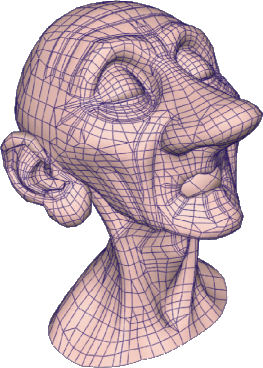
\includegraphics[height=5cm]{../images/geri_control}
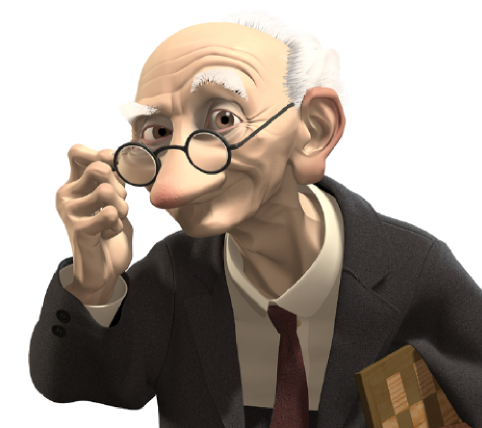
\includegraphics[height=5cm]{../images/geri2}
\caption[Pixar's Geri]{\label{fig:geri}Pixar's Geri, from their short film {\it Geri's Game}. A clay model of the head is digitised at particular points to obtain control points for a Catmull-Clark subdivision surface. Images taken from \cite{DeRose98}.}
\end{center}
\end{figure}
\citet{Pixar} have had some success in modelling surfaces using Catmull-Clark subdivision surfaces \cite{DeRose98}. For their short film {\it Geri's Game}, they created the head, hands and clothing of the main character by sculpting a clay model and capturing surface points with a CMM. These scanned points were then used as control points for the subdivision surface, illustrated in figure \ref{fig:geri}.

Alternatively, the dense scanned data can be retriangulated by hand. This allows a highly structured mesh to be constructed, but is very labour-intensive and can take many days of skilled work to remodel a complex surface. Nevertheless, this is the approach that is currently used by many animation houses, including \citet{Hensons}.

Animation systems that require an extremely accurate appearance, particularly for modelling realistic characters, utilise a highly layered anatomical approach. A skeleton model is built, and a muscle layer added on top. The densely scanned skin layer is mapped on top of this muscle layer, possibly with an extra layer in between to simulate body fat. Needless to say, this approach requires a great deal of skill and specialist knowledge to model, and a great deal of processing time to render and animate. The results, however, can be highly realistic.

\subsection{\label{sec:litreview:modeling:detail}Displacement Maps}

Fitting a polygonal or smooth surface to scanned data can represent the general shape of a model well, but fine surface details can be lost, as the surface cannot represent them at a high enough level of detail and remain efficient. However, a number of approaches have been suggested to store this residual detail in a displacement map, allowing an efficient yet detailed surface to be created. Much research has focused on hardware rendering of these representations (\cite{Gumhold99a}, \cite{Doggett00}), making it likely that the use of displacement maps will become more commonplace in the near future.

\citet{Krishnamurthy96} describe a method in which an object is scanned and converted into a dense polygon mesh. They then split this mesh into quadrilateral sections by manually drawing curves across the surface, reasoning that an automatic process will not create a surface suitable for animation. A B-Spline patch is then fitted to each section, creating a smooth representation of the model. The differences between this surface and the original polygon mesh are then encoded in a vector-valued displacement map for each patch, storing the fine details.

\citet{Lee00} define a similar method of representing complex datasets using displaced subdivision surfaces. A simplified version of a dense detailed mesh is generated using the MAPS algorithm \cite{Lee99}, which defines a control mesh for a Loop subdivision surface which approximates the scan data. At a number of sample points on the limit surface, a ray is cast along the surface normal, and an intersection calculated with the detailed polygonal surface. The distance between the two surfaces is then stored in a scalar-valued displacement map. Reconstruction is performed by calculating the the Loop subdivision of the control mesh, after which the stored displacement values are added to the new vertex positions. This representation allows fine surface detail to be encoded as a scalar field, making this a much more compact representation than the previous method. \citet{Jeong01} describe a method for building displaced subdivision surfaces directly from scanned surface data.

Lee's method is similar to that presented in this thesis, except that he uses a smooth base domain for his displacement maps, whereas we use a polygonal mesh surface. Lee also uses a low-to-high mapping to create his displacement maps, whereas we use a high-to-low mapping based on our intermediate detail layer representation. Both methods were developed concurrently, and we present our work as an alternative to this approach. A detailed comparison of the two methods is presented in section \ref{sec:conclusion:dispsubdiv}.

Such displacement map approaches store the fine details of a surface in an image format. \citet{Gu02} define a method which represents the complete mesh surface in this form, known as a {\it Geometry Image}. The dense dataset is first unwrapped automatically onto a 2D image plane. At each point in the image, the 3D position of the corresponding point on the dense surface is stored as a 3D vector, with the three components of the vector being stored in the three colour planes of the image. Normal images can also be created, which store the surface normal at each point in a similar fashion. This approach has the rather unique property that the geometry of the surface is stored in exactly the same manner as other surface features, such as texture and colour information.

\citet{Botsch03} describe a method related to displacement mapping that represents surfaces using {\it displacement volumes}, instead of using individual vectors for surface displacement. Rather than keeping the displacement between the base domain and the detailed surface the same, their approach preserves the volume of the surface under animation, giving a more realistic appearance in some circumstances.

\subsection{\label{sec:litreview:modeling:compression}Mesh Compression Techniques}

As well as simplifying complex datasets for animation purposes, it is sometimes useful to be able to keep those datasets in their original form, but still store and transmit them in an efficient manner. Progressive transmission of large datasets is also desirable, as a simplified version of the surface can be displayed quickly, followed by more complex versions \cite{King01}.

The field of mesh compression is young, and evolving rapidly. Most research falls into one of three categories. First, mesh-based approaches concentrate on the compression of geometric or topological data, by splitting the mesh surface into sections or strips. Examples include Topological Surgery by \citet{Taubin98}, which is used in MPEG-4, and the Edgebreaker method by \citet{Rossignac99}.

Alternatively, progressive approaches concentrate on reducing complex meshes into very simple ones, and then rebuilding the detailed surface one vertex at a time. \citet{Hoppe96} proposed an algorithm which simplifies mesh geometry through a series of edge collapses. This creates a low-resolution mesh which can be rebuilt one vertex at a time by reversing the edge collapse operation. \citet{Guskov00} define a similar method, which converts a retriangulated mesh into a simple base domain and a single floating-point coefficient per detail vertex. This floating point number represents a displacement from the base domain, and again allows a mesh to be rebuilt a single vertex at a time. The current state of the art in mesh compression, however, is proposed by \citet{Khodakovsky00}. Their method uses MAPS \cite{Lee98} to convert a dense mesh into a series of semi-regular approximations at different levels of detail. The refinement parameters between these approximation levels are then compressed with a wavelet-based encoding method, giving very high levels of lossy compression.

Increasingly, however, research is being carried out into the use of image methods for mesh compression. By representing meshes in an image-based form, either as displacement maps (\cite{Lee00}, \cite{Krishnamurthy96}), or as geometry images \cite{Gu02}, years of research into image compression can be applied to the efficient storage of large meshes. Such approaches are showing promise, but more research is yet to be done.

\subsection{\label{sec:litreview:modeling:software}Commercial Software}

There are a number of commercial software packages than incorporate some of the modelling techniques described above. 

{\it Remesh}, from \citet{3DScanners}, takes the approach of trying to ease the process of creating a structured polygon mesh from scan data. This would normally involve a large amount of manual joining of data points, as mentioned above, but Remesh allows the modeller to create a structured mesh from the a triangulated version of the original scan data without joining data points by hand. The modeller can draw {\it polylines} across the mesh, which are linked to define quadrilateral or triangular patches which are then subdivided to the desired resolution. This approach is described in more detail in section \ref{sec:scandata:creation:control:interactive}.

{\it Paraform} \cite{Paraform} implements the B-Spline patch modelling approach proposed by \citet{Krishnamurthy96}, described above. Geomagic {\it Shape} \cite{Geomagic} and Cyberware's {\it CySlice} \cite{Cyberware} create a similar representations based on NURBS patches. None of these packages deal with the animation of such models, however. They simply create a static mesh from the scan data, which can then be animated in a standard modelling package, such as 3D Studio MAX \cite{3DSMAX} or Maya \cite{Maya}.

\section{\label{sec:litreview:animation}Animation Techniques}
One of the most important applications for models built from scanned data  is the creation of models that can be animated, for use in special effects or games. The ability to scan rigid objects is useful, but ideally, we want to be able to create models that are non rigid, and that can move and bend. In short, we should be able to easily create {\it deformable} models.

\subsection{\label{sec:litreview:animation:skeleton}Articulation Structures}
\nomenclature{\bf Segment}{A rigid link between joints in a skeleton structure, for instance representing a bone in a human body.}
\nomenclature{\bf Joint}{A node in a skeleton structure, which can be rotated or transformed to provide control over the pose of the skeleton. }
\nomenclature{\bf End Effector}{A node in a skeleton structure which represents the end of the hierarchy, normally corresponding to feet, fingertips, and so on. }
\begin{figure}
\begin{center}
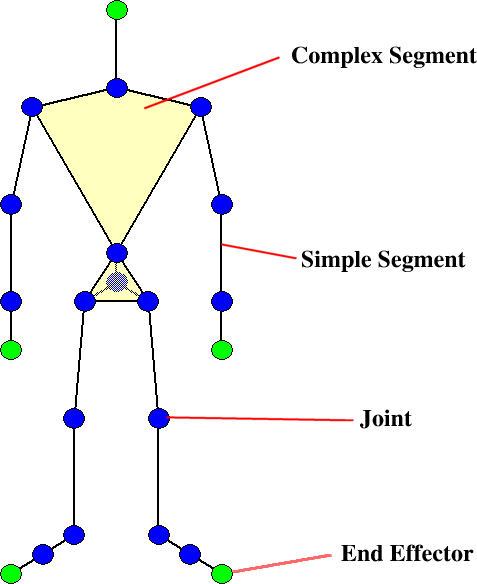
\includegraphics[height=7cm]{../images/skeleton_nosites}
\caption[Skeleton Structure]{\label{fig:skeleton} Skeleton Structure. A skeleton consists of a set of joints connected by rigid segment links.}
\end{center}
\end{figure}
Keyframing techniques are often used for model animation, but these can only represent a limited set of pre-calculated motions for a surface. In cases where arbitrary motions are required, {\it skeletal animation} is used. This uses a flexible articulation structure to drive motions of a surface or skin layer. A skeleton structure consists of a hierarchical series of {\it joints}, which are connected together by rigid links known as bones or {\it segments}, as shown in figure \ref{fig:skeleton}.

Skeletal animation is normally driven by joint rotations, in which a rotation is applied to each joint and its children. For instance, if a shoulder joint of a skeleton is rotated, the entire arm below that point rotates with it. Each joint rotation is applied incrementally, so the position of an individual segment will be defined by the rotations of all of the joints above it in the hierarchy. Rotation data for joint animation can be obtained in a number of ways, from manual location, through inverse kinematics systems (in which the modeller simply positions an {\it end effector}, for instance a foot, and the required joint rotations are calculated automatically), to motion capture systems that record the real-world movements of a human subject.

As well as the skeleton structure itself, the surface of a deformable model must be affected by transformations of the various joints. This is carried out by defining a method of attaching the surface to the skeleton, by associating parts of the surface with the skeleton in some way. The surface then deforms as the skeleton is moved. The most common methods of performing this association and deformation are described below.

\subsection{\label{sec:litreview:animation:geometric}Geometric Methods}

The first class of deformation techniques we will cover are geometric approaches. These type of methods have the advantage that the skin layer is operated on only by simple geometric transformations, as opposed to complex physical or anatomical simulations. This makes them comparatively cheap to calculate, and hence more appropriate for real-time applications. 

\subsubsection{\label{sec:litreview:animation:geometric:ssd}Skeletal Subspace Deformation}

The simplest method of deforming a skin model with a skeleton is to use vertex blending, or {\it Skeletal Subspace Deformation} \cite{Akenine02}. This technique has never been officially published, but related methods have been presented by \citet{Komatsu88}, and \citet{Magnenat-Thalmann88}. The technique is also used in many commercial animation packages.

\begin{figure}
\begin{center}
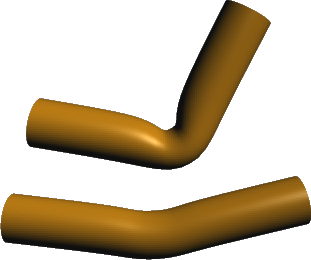
\includegraphics[width=7cm]{../images/bend}
\caption[Skeletal Subspace Deformation]{\label{fig:ssd} Skeletal Subspace Deformation. Simple deformation techniques suffer from collapse around joints, as well as during twisting.}
\end{center}
\end{figure}

SSD methods simply assign each vertex in a skin layer to one or more of the skeleton segments, along with a weight for each segment. The deformed position of the vertex is the weighted average of the original position after application of the transformation for each segment. This method can give realistic results, but can require much user interaction to define the vertex weights. It can also be unpredictable, and not all deformations can be represented in this fashion. Classic SSD problems include thinning around joints (shown in figure \ref{fig:ssd}), and the complete collapse of geometry under segment-aligned rotations.

\citet{Lewis00} describe a method which uses aspects of both keyframed and SSD animation. They define a set of poses for a surface, with user-defined geometry for each. Skeletal animation can then be applied, and the deformed surface is generated by shape interpolation between these key poses.

\subsubsection{\label{sec:litreview:animation:geometric:ffd}Free-Form Deformations}
Free-Form Deformation (FFD), proposed by \citet{Sederberg86}, is a method of deforming arbitrary objects. The object to be deformed is embedded in an FFD block, which is in fact a tricubic Bezier hyperpatch, an extension to three dimensions of the spline patches described in section \ref{sec:litreview:surfaces:smooth:curved}. In order to deform the surface, the hyperpatch control points are moved, thus changing the geometry of the hyperpatch and the object within it.

The FFD method has been extended by \citet{Coquillart90} to allow arbitrarily shaped FFD spaces to be created by combining a number of FFD lattices, a technique known as Extended Free-Form Deformation (EFFD). \citet{MacCracken96} further extend FFD to allow lattices of arbitrary topology.

\citet{Chadwick89} present an effective method of using FFDs for character animation, known as {\it Critter}. This system represents a deformable character as three layers; an articulated skeleton structure, a muscle layer (represented as a set of FFD blocks), and a skin layer, which is deformed by the FFD muscle layer. The muscle layer is constructed by placing an FFD block around each joint (called a {\it flexor}), and also one along each segment (called a {\it tendon}). The control points within each FFD block are also controlled by movements of the joints. Flexors are scaled orthogonally to the segment to simulate muscle inflation, while the faces of the tendons are rotated according to the rotation of closest joint. The faces of the FFD blocks are held together, so that when a joint bends, both the flexor and tendon blocks are affected.

\subsubsection{\label{sec:litreview:animation:geometric:bspline}Hierarchical B-Spline Models}
\citet{Forsey91} describes a method of constructing articulated characters using a hierarchical B-Spline representation. Control points for a set of B-Spline patches are attached to the segments of the skeleton, so that the smooth surface follows the movements of the joints. This is enough for gross movement of the surface, but detailed movements around the joints cannot be represented in this way. Therefore, the area around the joint is split into a number of subsegments, between which the rotation angle is divided up, giving a smoother joint in the skeleton. Extra control points can then be added to these, giving a smoother surface in joint regions.

\subsubsection{\label{sec:litreview:animation:geometric:metaballs}Metaballs}
\citet{Shen95} describe a method of modelling shapes using {\it metaballs}, which are fixed to the a skeleton to build up the deformable surface, simulating the appearance of muscles and so on. There is no precise relationship between metaballs and real muscles, however, making the modelling process completely subjective on the part of the modeller. The parameters of the metaballs, such as major and minor axes, are controlled by joint angles, so that the metaballs change shape as the skeleton moves. After deformation, the implicit surface of the combined metaballs is converted into a polygonal representation for display. At regular intervals along the segments of the skeleton, rays are cast orthogonally from the segment to the surface of the metaball body. The positions of the intersections with the surface become the vertices of the polygonal model. The polygonal model is therefore structured in contours, with a consistent number of vertices around each contour. 

This approach, though it produces realistic results, is computationally expensive, as the skin layer is recalculated completely every time the body is moved. \citet{Thalmann96} therefore propose an improved method, in which the polygonal surface of the model is generated only once after modelling, and all deformation is performed by rotating the contours of the polygonal model according to joint movements. This deformation method is fast enough for realtime calculation, and has been used to implement surface deformation in VRML by \citet{Babski99}.

\subsection{\label{sec:litreview:animation:physics}Anatomical and Physical Methods}
If highly realistic results are required, more complex anatomical or physical deformation techniques can be used. Physical methods of character animation involve some aspect of physics simulation, often a simple spring-based model. Anatomical methods construct a model that has several highly realistic layers, such as multiple muscles, fat and skin layers, and as such are almost always too expensive for realtime animation. Also, such models are very complex to build, and require the modeller to specify multiple weighting parameters dependent on the muscle or skin area being modelled. This is a very difficult process, and is not suited to rapid construction of models.

\subsubsection{\label{sec:litreview:animation:physics:layered}Layered Deformable Bodies}
\citet{Gascuel91} propose a method that uses three layers to construct a deformable model. The bottom layer is a normal skeleton structure, to which a physical spring simulation layer is attached. Springs are attached to the skeleton at one end, allowing the other end to move freely along the axis of the spring. Extensions of springs are propagated to other nearby springs, so that deformations are consistent within a small area. The free end of the spring is used as a control point for a B-Spline based skin layer. This approach is simple enough to compute in a reasonable time. The springs also handle collisions between body parts, so that realistic deformations around the inside of joints are obtained without self-intersection of the surface.

\subsubsection{\label{sec:litreview:animation:physics:anatomical}Anatomical Modelling}
A method for body modelling based on anatomical principles is proposed by \citet{Nedel98}. Their models consist of a large number of physically accurate muscles attached to accurate points on a skeleton model. Needless to say, the modelling effort required to create this kind of model is very large. The models are, however, based in reality, so the modelling process is not as subjective as for the metaball method described above. Upon movement of the skeleton, the muscles deform in a physically accurate way. The skin model is then generated after each movement in the same way as Shen's method for metaball modelling, by casting rays from the segments out to the surface of the muscles and generating contours for a polygonal model.

\subsubsection{\label{sec:litreview:animation:physics:leman}LEMAN}
The LEMAN (Layered Elastic Model ANimation) system, developed by \citet{Turner93}, combines aspects of geometric, physics-based and anatomical methods. It defines a model constructed from many layers, each with their own set of properties and deformation method. There are four layers, the skeleton, muscle, fat and skin layers. The skeleton layer is a standard skeleton structure. The muscle layer above this is composed of parametric smooth surfaces, such as spheres or superquadrics, which are deformed using a simple geometric deformation method dependent on joint angles and the pose of the skeleton. The fat layer is simply modelled as a constant thickness, to hold the skin and muscle layers apart. Finally, the skin layer is a physics-based model of an elastic surface, which is deformed by the muscle layer. The deformations of the muscle layer are used to calculate forces, which are applied to the skin layer using a simplified spring model, using springs that are attached to the muscles at one end and the skin at the other. The springs are subject to a number of parameters that govern how the skin moves over the muscle in different areas of the surface.

\subsection{\label{sec:litreview:animation:vrml}Character Animation in VRML}
As the use of 3D graphics on the Internet grows, demand is increasing for high-quality animation of articulated characters that can be represented in standard formats and displayed on consumer hardware. VRML97 \cite{VRML97} is currently the dominant format for 3D models on the Internet, so we will look briefly at how character animation is currently performed in this language. The H-Anim 1.1 specification \cite{HANIM99} defines a method for representing articulated humanoid characters in VRML, but due to the limitations of VRML97 itself, it cannot represent deformable models. H-Anim 1.1 models are constructed from separate rigid segments, which are unrealistic around joints, and have problems of surface and texture discontinuity.

At the start of this research, little work had been done on the creation of seamless deformable models in VRML. Only two systems were known of, though one of these, by Lionhearth \cite{Lionhearth}, has never been released to the community. The only method that had been published is described by \citet{Babski99}, and is an implementation for VRML of the contour-based deformation proposed by \citet{Thalmann96}, and described in section \ref{sec:litreview:animation:geometric}.
\begin{figure}
\begin{center}
\begin{tabular}{cc}
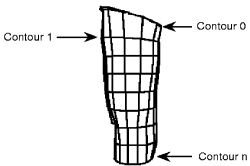
\includegraphics[height=3.5cm]{../images/babski_contours} &
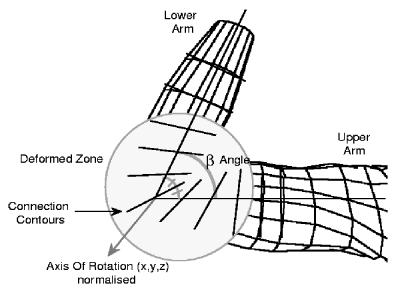
\includegraphics[height=3.5cm]{../images/babski_deformation} \\
{\it(a)} & {\it(b)}
\end{tabular}
\caption[Contoured models for VRML animation]{\label{fig:babskimodels}Contoured models for VRML animation. (a) Model structure for a single body segment. (b) Contour-based deformation around joints. Images taken from \cite{Babski99}.}
\end{center}
\end{figure}
Each segment of the model is defined as a set of contours (see figure \ref{fig:babskimodels}a). The last contour of one segment is also the first contour of the next, ensuring that the body appears seamless. When a joint rotates, the contours near joints are rotated by different amounts, varying from no rotation to half of the rotation of the joint, as shown in figure \ref{fig:babskimodels}b. This contour rotation is applied on both sides of a joint, preserving the model's seamless appearance. The deformation can be executed in real time, due to the efficiency gained by rotating complete contours at once. However, the deformation method suffers from thinning of segments due to the contour rotation, and also cannot handle segments that have more than two joints (e.g. the pelvis).

\section{\label{sec:litreview:conclusion}Conclusion}

In this section we have reviewed the state of the art across all stages of the process of creating models for animation. We have seen that scanning hardware produces accurate surface data, but at far too high a density, and in too unstructured a format to be directly usable. Various modelling techniques have been developed to ease the use of such models, but most require a large amount of manual intervention. A more highly automated method for the creation of these models would be highly desirable, and make the content creation process much easier.

We therefore move on to the description of our layered animation method, which provides an efficient and highly automated method of animating dense scanned surface data.
